\subsection{Peak Ratio}\label{subsec:peakratio}

The Sandvine Reports show that although the mean traffic demand has remained
stable for the past few years, demand during prime-time hours has increased
drastically~\cite{sandvine20141h}. These reports present a good view 
into aggregate usage patterns over a month, however they neglect to analyze usage
characteristics per subscriber.
We measure the disparity between the daily 95 percentile of the peak and 
mean usage of each household, and call this the \emph{Peak-Ratio}.

\begin{figure}[t]
\begin{minipage}{1\linewidth}
\centering
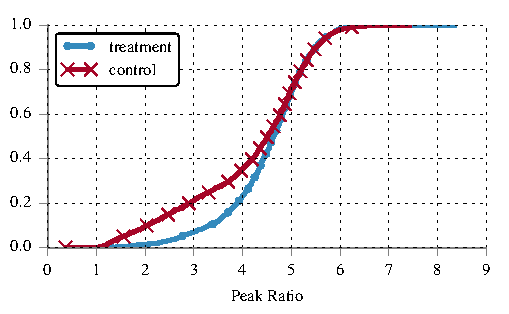
\includegraphics[width=1\linewidth]{figures/peakratio_cdf_mean-devices.pdf}
\caption{Distribution of the average peak ratio per subscriber in the treatment and 
control groups.}
\label{fig:CDF-peak-ratio-mean}
\end{minipage}
\end{figure}

Figure~\ref{fig:CDF-peak-ratio-mean} plots the peak-ratio for each 
subscriber in \treatment{} and \control{}. The median peak
ratio for subscribers from the higher and lower tier is 4.64 and 4.51
respectively. 40\% of the subscribers in bothe groups have peak ratios
greater than 5, and have similar distributions. 60\% of the subscribers
in the control and treatment group have peak ratios less than 5, however,
the peak ratio of subscribers in the higher tier is more than that of the lower
tier.

The decrease in prime time ratio by volume, and a consistent increase
in the peak ratio per subscriber indicates the following: subscribers in the treatment
group have high peak:mean ratio than those in the control group. However, (1) their
traffic demand is low and they do not affect total traffic durin prime-time significantly,
or (2) their demand is high but mostly during non-prime-time hours.

Further analysis showed that on weekdays, peak ratios in the treatment group are higher
than the control group, whereas on weekends peak ratios for both \control{} and \treatment{}
group are similar.